% \section{Requirementsanalysis}

Die Anforderungsanalyse ist ein entscheidender Schritt im Software-Entwicklungsprozess, der dazu beiträgt, die Bedürfnisse der Nutzer zu identifizieren und zu verstehen. Um jedoch die Bedürfnisse der Nutzer vollständig zu verstehen, ist es notwendig, eine detaillierte Analyse der Geschäftsanforderungen durchzuführen. Das Value Proposition Canvas bietet dabei eine effektive Methode zur Identifizierung der Kundenbedürfnisse und zur Entwicklung von wertvollen Produkten und Services. Dieses Kapitel befasst sich mit der Anforderungsanalyse mit dem Hilfsmittel des Value Proposition Canvas.

\subsection{Value Proposition Canvas}

Die Anforderungsanalyse nach dem Value Proposition Canvas ist ein Prozess, bei dem die Bedürfnisse und Anforderungen der Kunden identifiziert und dokumentiert werden, um sicherzustellen, dass das Unternehmen Produkte oder Dienstleistungen anbietet, die einen hohen Nutzen für die Kunden bieten.

\begin{figure}
    \centering
    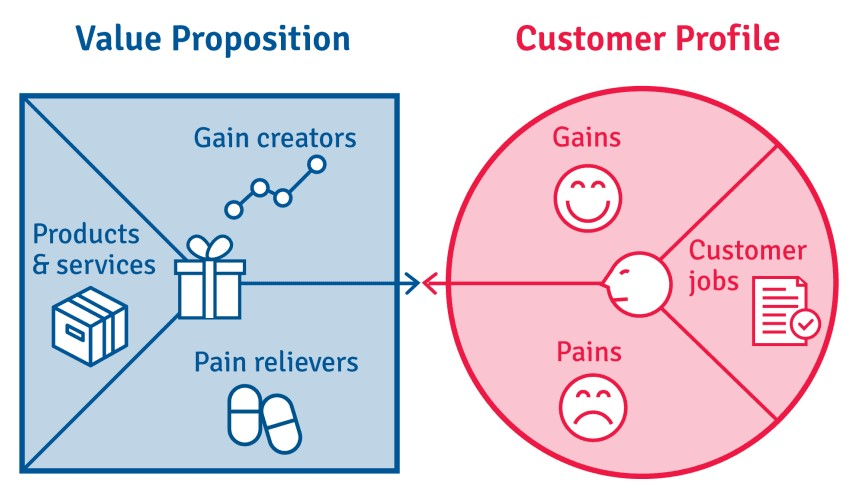
\includegraphics[width=0.6\textwidth]{figures/andre/valuepropositioncanvas.jpg}
    \caption{Value Proposition Canvas}
    \label{fig:valuepropositioncanvas}
\end{figure}

Der Value Proposition Canvas besteht aus zwei Hauptbereichen:

\begin{itemize}
    \item[1.]	Der Kundenprofilbereich: In diesem Bereich identifizieren Sie die Bedürfnisse und Anforderungen Ihrer Zielgruppe und erstellen ein detailliertes Profil der Kundenperspektive.
    \item[2.]	Der Value-Map-Bereich: In diesem Bereich legen Sie fest, wie Ihr Produkt oder Ihre Dienstleistung den Kundenbedarf erfüllt und welche Vorteile es im Vergleich zu anderen Lösungen bietet.
\end{itemize}

\subsection*{Vorgehensweise}

Um eine erfolgreiche Analyse nach dem Value Proposition Canvas durchzuführen, sollten folgende Schritte beachtet werden:

\begin{itemize}
    \item[1.] Kundenprofilbereich 
    \begin{itemize}
        \item Identifizierung der Bedürfnisse und Herausforderungen der Zielgruppe
        \item Definierung der Kundenperspektive und Erstellen eines Profils für die Zielgruppe
    \end{itemize}
    \item[2.] Value-Map-Bereich
    \begin{itemize}
            \item Definition der Produkte oder Dienstleistungen, die angeboten werden sollen
            \item Festlegung der Vorteile, die das Produkt gegenüber anderen Konkurrenten bieten könnte
            \item Sicherstellung, dass die Bedürfnisse der Zielgruppe erfüllt werden
    \end{itemize}
\end{itemize}

\subsection{Personas und Zielgruppe}
Zu Beginn des Projekts wurde bereits die initiale Zielgruppe definiert. Da eine Social Media Plattform grundsätzlich ein potentiell sehr breites Spektrum an Nutzern besitzt, wurde die Entscheidung der Zielgruppe anhand dem bestmöglichen erreichen vieler Menschen definiert: Junge Erwachsene und Vereine - unter Betrachtung eines eher ländlicheren Landkreises.

Junge Erwachsene sind in der Regel affin und offener für den Umgang mit Technik, bei Erfolg der Plattform könnten diese wiederum über persönliche Kontakte und Werbung weitere Nutzer auf die Plattform ziehen. Vereine besitzen in der Regel bereits ein Netzwerk und bieten gleichzeitig die Möglichkeit, Menschen mit ähnlichen Interessen miteinander zu verknüpfen.

\subsection{Profile}
Um die Zielgruppen abbilden zu können, wurden insgesamt 4 Profile definiert, diese wurden nach dem Value Proposition Canvas analysiert und daraus jeweils Features abgeleitet. Diese sollen im Folgenden beschrieben werden:
\subsection*{Musikverein}
Beim Musikverein wird angenommen, es handelt sich um einen existierenden Verein mit einer funktionierenden Vorstandschaft und einer lebhaften Mitgliedschaft.
Dieser hat nach dem Value Proposition Design die folgenden Eigenschaften:


\subsection*{Alleinstehender Erwachsener Mann, frisch zugezogen}
Bei dieser Person handelt es sich um einen jungen alleinstehenden Mann, der erst wenige Wochen im Ort wohnt um eine neue Arbeit anzutreten. Dieser kennt nur das nötigste, ist zwar technikaffin, aber handwerklich nicht sonderlich begabt.

\subsection*{Alleinstehende Frau mittleren Alters}
Diese Frau ist alleinstehend, geschieden und Vollzeit berufstätig. Sie hat 2 jugendliche Kinder welche bei ihr wohnen und ist auf der Suche nach einem neuen Lebenspartner. Sie ist Mitglied in einem Gartenbauverein in der Gemeinde.

\subsection*{Junges Pärchen}
Mit diesem Profil soll ein junges Pärchen abgebildet werden. Diese sind beide Mitte 20 und leben in ihrer ersten gemeinsamen Wohnung. Beide sind voll berufstätig und daher zeitlich sehr eingeschränkt. Beide studieren und würden ihr wissen gerne mit anderen teilen.

\subsection{Abgeleitete Features}
Zusammen mit den Zielen aus der Aufgabenbeschreibung sowie den Erkenntnissen aus der Kundenanalyse des vorange-gangenen Kapitels wurden folgende Features abgeleitet.

\subsubsection{Persönliche und Vereinsprofile}
\label{sec:abgeleitetefeatures}
Im Vordergrund einer Social Media Plattform steht die Darstellung der eigenen Person. Daher war die Grundlage für die Plattform die Implementierung von Profilen.
Die Anforderungen für das Profil waren, sich kurz und knapp selbst beschreiben zu können. Die Einfachheit der Bedienung und damit für potentielle Profiländerungen sollte gegeben sein. Mit den Nutzerprofilen sollte nur das Interesse an der Person oder dem Verein geweckt werden, um im nächsten Schritt einen direkten Kontakt über die Chatfunktion zu ermöglichen.
Ein Schlüsselelement der Plattform ist das sogenannte Tag-System, ähnlich dem bekannten Hash-Tag von Netzwerken wie bspw. Twitter. Über die Tags kann ein Nutzer seine Hobbys und Interessenfelder kurz und knapp angeben.
Zusätzlich zum Tag sollte auch die Möglichkeit gegeben sein, sich selbst über einen Freitext beschreiben zu können.
Die Option ein Profilbild hochladen zu können ist ebenfalls eines der Basis-Anforderungen die das System haben muss.

\begin{figure}[ht!]
    \centering
    
\includegraphics[width=0.6\textwidth]{figures/andre/beispielprofil.jpg}
    \caption{Beispielprofil}
    \label{fig:beispielprofil}
\end{figure}

In der obigen Abbildung ist ein Beispielhaftes Profil zu sehen. Es kann kurz und knapp auf das Thema der Organisation, in diesem Fall ein Fanclub über Arnold Schwarzenegger, abgeleitet werden. Des Weiteren sind auf dem Profil auch die erstellten Beiträge zu finden, ebenso wie eine Möglichkeit direkten Kontakt aufnehmen zu können. 

\subsubsection{Chats und Chaträume}
Ebenso obligatorisch wie die Profile ist auch die Chatfunktion, die zur Kontaktaufnahme unabdingbar ist. 
Auch hier stand wieder die Einfachheit im Fokus. Dies kann dadurch begründet werden, dass die Plattform nur zum Kennenlernen und Vernetzen der Menschen gedacht ist.
Ebenfalls soll die Möglichkeit bestehen, Gruppenchats zu erstellen. Dadurch kann man sowohl den Privatpersonen als auch Vereinen eine Möglichkeit geben sich in Gruppen zu organisieren. 

\begin{figure}[ht!]
    \centering
    \includegraphics[width=0.6\textwidth]{figures/andre/chatsundchaträume.jpg}
    \caption{Chats in Digital Dahoam}
    \label{fig:chatsundchaträume}
\end{figure}

\subsubsection{Beiträge, Veranstaltungen und Events}
Ebenfalls wichtig zur Kommunikation und Selbstdarstellung ist das Erstellen von Beiträgen. 

Aufgrund der Anforderungen wurden hierfür 4 Kategorien an Beiträgen herauskristallisiert:

\begin{itemize}
    \item	\textbf{Angebot} Man bietet etwas an, wie bspw. Hilfeleistung bei handwerklichen Tätigkeiten
    \item	\textbf{Anfrage} Hilfegesuch zu einem bestimmten Thema
    \item   \textbf{Information} Allgemeine Mitteilung
    \item 	\textbf{Veranstaltung} Teilen einer bevorstehenden Veranstaltung
\end{itemize}

Durch diese Kategorien können grundlegend die meisten Bedürfnisse zufriedengestellt werden. Es gibt sowohl die Möglichkeit, sich auszutauschen, als auch die Möglichkeit aktiv bzw. passiv nach Hilfe in der Nachbarschaft zu suchen bzw. diese anzubieten. Vereine können ihre Events mit der Öffentlichkeit teilen.

\subsubsection{Marktplatz und Entdecken}

Aufbauend auf den Beiträgen soll der Nutzer die Möglichkeit haben, gezielt nach eben jenen suchen zu können. Dies soll über das Explorationstool der Website ermöglicht werden.
Die Anforderungen hierfür waren, dass grundsätzlich nach allem und jedem gesucht bzw. gefiltert werden kann, anhand der zugewiesenen Tags. Dadurch kann dem Nutzer ermöglicht werden, auch wirklich nur die Beiträge zu sehen, die ihn auch Interessieren.
Des Weiteren sollten basierend auf demselben Prinzip (Tags) auch Personen gefunden werden können. Es wurde hierbei bewusst auf eine Klarnamensuche verzichtet, mit dem Ziel so möglichst viele neue Bekanntschaften zu ermöglichen. 

\begin{figure}[h!]
    \centering
    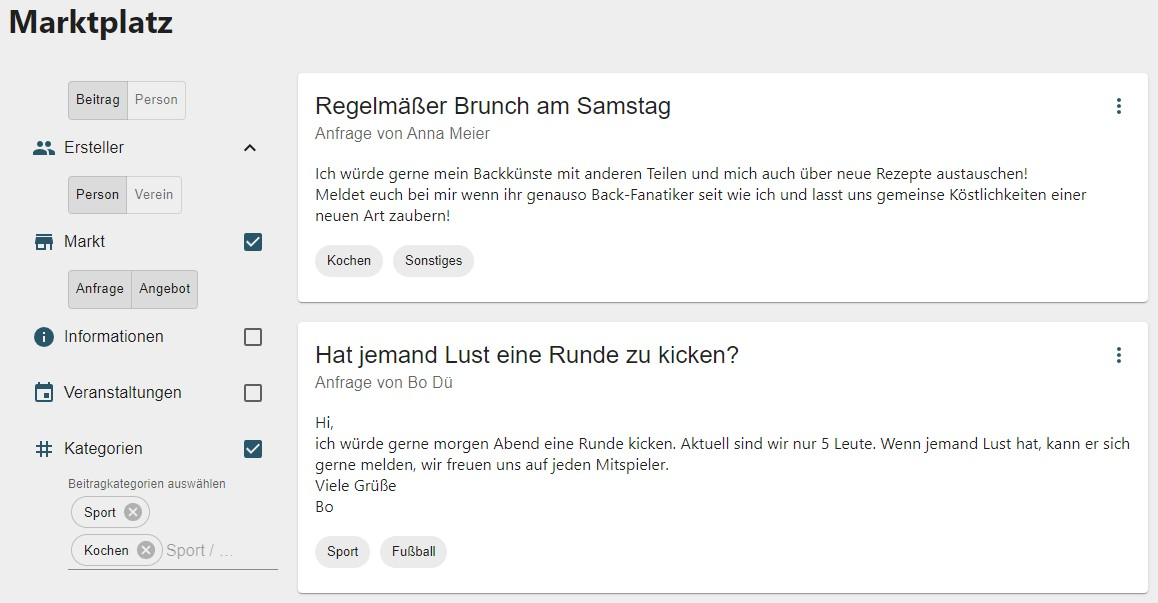
\includegraphics[width=0.6\textwidth]{figures/andre/marktplatzvondigitaldahoam.jpg}
    \caption{Marktplatz von Digital Dahoam}
    \label{fig:marktplatzvondigitaldahoam}
\end{figure}

\subsubsection{Persönlicher Merkzettel}
Als weiteres Feature sollte ein sog. Merkzettel implementiert werden. Dieser stellte sich als unabdingbar notwendig heraus für den Fall, dass ein Nutzer eine Veranstaltung sieht an der er interessiert ist und für später merken möch-te.
Aus dieser Anforderung wurde das allgemeine Feature des Merkzettels implementiert, sodass grundsätzlich die Möglichkeit gegeben ist, sich alle Beiträge merken zu können. Ähnlich wie beim Marktplatz kann auch hier nach den verschiedenen Beitragstypen gefiltert werden.

\begin{figure}[ht!]
    \centering
    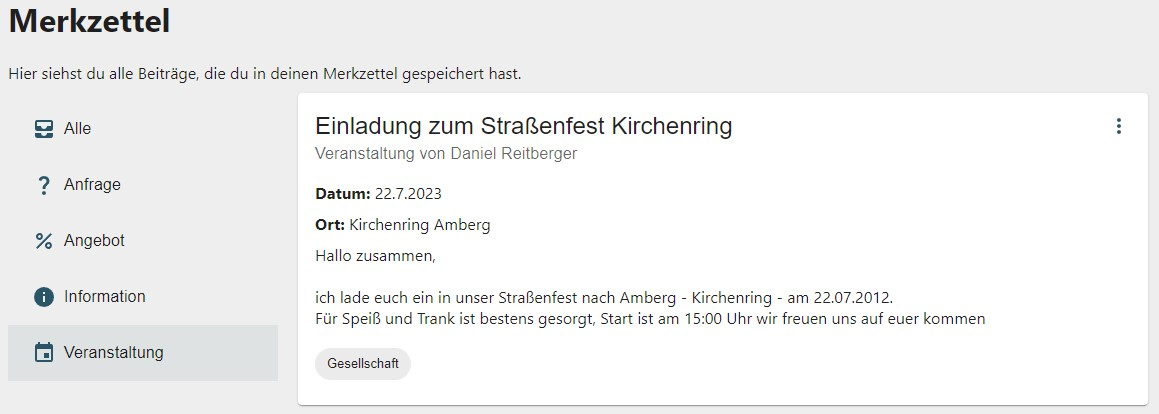
\includegraphics[width=0.6\textwidth]{figures/andre/merkzettel.jpg}
    \caption{Merkzettel}
    \label{fig:merkzettel}
\end{figure}